%!TEX root = ../thesis.tex
%*******************************************************************************
%****************************** Third Chapter **********************************
%*******************************************************************************
\chapter{Applications}

% **************************** Define Graphics Path **************************
\ifpdf
    \graphicspath{{Chapter3/Figs/Raster/}{Chapter3/Figs/PDF/}{Chapter3/Figs/}}
\else
    \graphicspath{{Chapter3/Figs/Vector/}{Chapter3/Figs/}}
\fi

In the first two chapters I have provided an overview of the theoretical basis of my work and placed it within the history of related approaches.
Here, I will demonstrate how the methods I develop can aid biological insight in a number of species domains.
To do so, I will use methods described in chapter 2 as implemented in {\tt vg}.

The small genome of \emph{Saccharomyces cerevisiae} and ready availability of sources for pangenomic data models made it very useful to my development of {\tt vg}.
I do so for a variety of pangenome constructions and also a variety of read lengths.

However, much interest in bioinformatics is with larger genomes, specifically human.
I use evaluations based on the human genome to validate the ability of {\tt vg} to scale to large genomes.
Through simulation and the analysis of real genomes, I show that {\tt vg} yields exactly the same quality of alignment as {\tt bwa mem} with runtime within five to ten-fold slower.
I develop a variation graph for the reference-guided genome assemblies from the HGSVC project and demonstrate the strong effect of reference bias in ChIP-seq.

One context where reference bias has very significant effects is in the analysis of ancient DNA (aDNA).
Here short reads and high intrinsic error rates encourage a high rate of reference bias.
I show that alignment against a pangenome graph ameliorates this issue.

{\tt vg} can be applied to any kind of variation graph.
To demonstrate the utility of this, I use de Bruijn assemblers to generate reference variation graphs.
I recreate a classical pangenomic analysis of core and accessory pangenome by analyzing the coverage of alignments mapped to an assembly graph built from 10 \emph{Escheria coli} strains.
{\tt vg} enables the full length alignment of reads to a complex assembly graph built from an arctic viral metagenome.

Finally, I demonstrate that the data models and indexes in {\tt vg} are capable of encoding splicing graphs, and that aligning to these splicing graphs allows the direct observation of the transcriptome.

\section{Yeast}
%*0.5p 0.5h*

\emph{Saccharomyces cerevisiae}, commonly known as baker's or brewer's yeast due to its gastronomic applications, has long been among the most important model organisms in biology, and its small genome attracted some of the first population scale whole genome surveys of variation to be undertaken using low-cost sequencing.
The genome of \emph{S. cerevisiae} was the first eukaryotic genome sequenced, in 1996 \cite{goffeau1996life}.
Resequencing studies followed that used \emph{cerevisiae} as a model system to understand genome evolution.
The Saccharomyces Genome Resequencing Project (SGRP) \cite{litisgrp}, which used low-coverage capillary Sanger sequencing to generate a population survey for \emph{cerevisiae} can be seen as a precursor to the 1000GP, in its use of low-coverage sequencing and imputation to establish the panel\footnote{\url{https://www.sanger.ac.uk/research/projects/genomeinformatics/assets/sgrp_manual.pdf}}.
A followup project, the SGRP2, resequencing and whole genome assembly of high coverage, low cost Illumina sequencing to establish that the greater phenotypic diversity in \emph{S. cerevisiae} relative to its wild relative \emph{S. paradoxus} is likely due to structural variation (as measured by presence/absence and copy number) rather than SNP diversity \cite{bergstrom2014high}.
Recently, whole genome \emph{de novo} assembly with long single-molecule reads has further refined this conclusion by demonstrating that the structural diversity is non-uniformly distributed through out the genomes of \emph{S. cerevisiae}, concentrating in subtelomeric regions \cite{yue2017contrasting}.
In this section, I use data from independent sequencing of the UK's National Center for Yeast Collections (NCYC) as well as long reads from \cite{yue2017contrasting} to demontrate the capabalities of {\tt vg} and compare the utility of various variation graph models built from these population surveys.

\subsection{A SNP-based SGRP2 graph}
%*1p 1h*T
%I consider only \emph{S. cerevisiae}, using the SGD reference genome and the SNP variation results from the SGRP2.
The earliest rigorous testing of {\tt vg}'s alignment method was against a variation graph constructed from the SGRP2's released VCF for \emph{S. cerevisiae}\footnote{\url{http://www.moseslab.csb.utoronto.ca/sgrp/data/SGRP2-cerevisiae-freebayes-snps-Q30-GQ30.vcf.gz}}.
This early population resequencing project produced a VCF including only SNPs, yet using it already presented problems typical even when working with larger scale genomes.
The transposable elements in the genome generate rich patterns of repeats which make alignment difficult and require the development mapping quality.
Dense variation is also present in the results and this necessitates the application of pruning strategies to the graph to mask out high-complexity regions for indexing.
Mistakes in the mapper could be readily observed and testing could easily be done on a laptop, whereas larger genomes require longer runtimes for indexing and larger servers in order to support the indexes during alignment.

The SGRP2 graph can be built and indexed in around 10 minutes on a commodity compute server, including the construction of the GBWT index and the generation of an order-256 GCSA2 index using a pruned and refilled version of the graph.
The graph contains exactly the number of bases in the SGD\_2010 reference plus the number of SNP alternate alleles in the SGRP2 VCF: 12163423 + 243629 = 12407052.
The graph itself is 23MB on disk, in contrast to that of the SGD\_2010 reference, which is only 7.6MB.
Much of this difference is due to the larger number of entities required by to represent the variation-containing graph.
The SGD\_2010 graph is linear, with a gap for each chromosome, and contains 380,115 nodes and 380,097 edges, while the SGRP2 graph contains SNPs and must be represented with 714,533 nodes and 969,690 edges.
Note that by default, GCSA2 indexing works on nodes with a maximum length less than 1024, and {\tt vg map} performs better if the maximum node size is limited further, with 32bp usually the standard maximum length in experiments I will present here.
The resulting indexes also differ in size, with the SGRP2 graph's {\tt xg} index requiring 71MB, while the SGD\_2010 graph's only 38MB.
The GCSA index for the SGRP2 graph is substantially larger, at 220MB, in contrast to only 50MB for the linear reference, which reflects the greater complexity required to include all the recombination in the pruned and haplotype re-filled graph used for indexing.

To validate that the SGRP2 reference is a closer match to real read sets, I then mapped subsets of reads from \emph{cerevisiae} samples that were in the NCYC collection but were not part of the SGRP2.
I aligned 100K read pairs from each of 12 samples ($N=2.4$M total reads) to both the SGD\_2010 reference graph and the SGRP2 pangenome graph.
For each read, we can compare the alignment score and identity between the two graphs to evaluate the gain provided by using the pangenome as a reference.
When we map the real reads from new strains not used to build the graph, 24.5\% of the reads map better to the pangenome than to the linear reference.
A small fraction of reads (0.46\%) map better to the linear than to the pangenome graph, which could result from changes in paired alignment rescue, the effects of the pruning process, the slightly different minimum MEM size calculated for the two graphs, or errors in the SGRP2.
%Although differences in the relative benefit of using the SGRP2 pangenome appear between samples, they are minor and not apparently systematic (Figures \ref{subfig:NCYC_score_diff_hist} and \ref{subfig:NCYC_id_diff_hist}).

\begin{figure}[htbp!] 
  \centering
  \begin{subfigure}[t]{0.49\textwidth}
    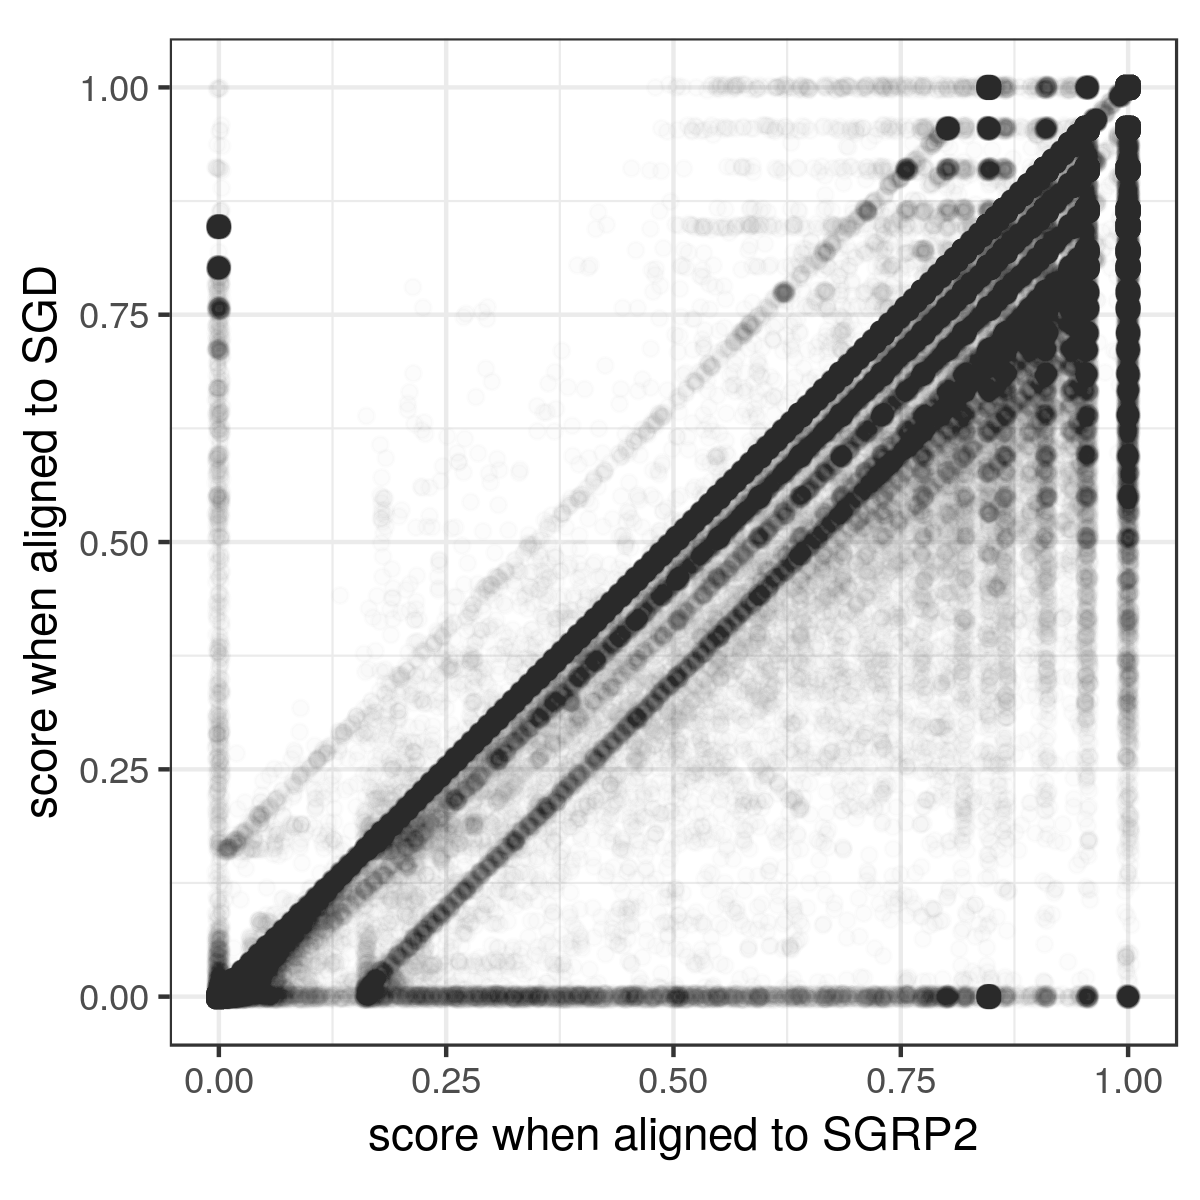
\includegraphics[width=1.0\textwidth]{Chapter3/Figs/NCYC_SGRP2_SGD_comparison_score.png}
    \caption{Alignment score} \label{subfig:NCYC_score}
  \end{subfigure}
  \begin{subfigure}[t]{0.49\textwidth}
    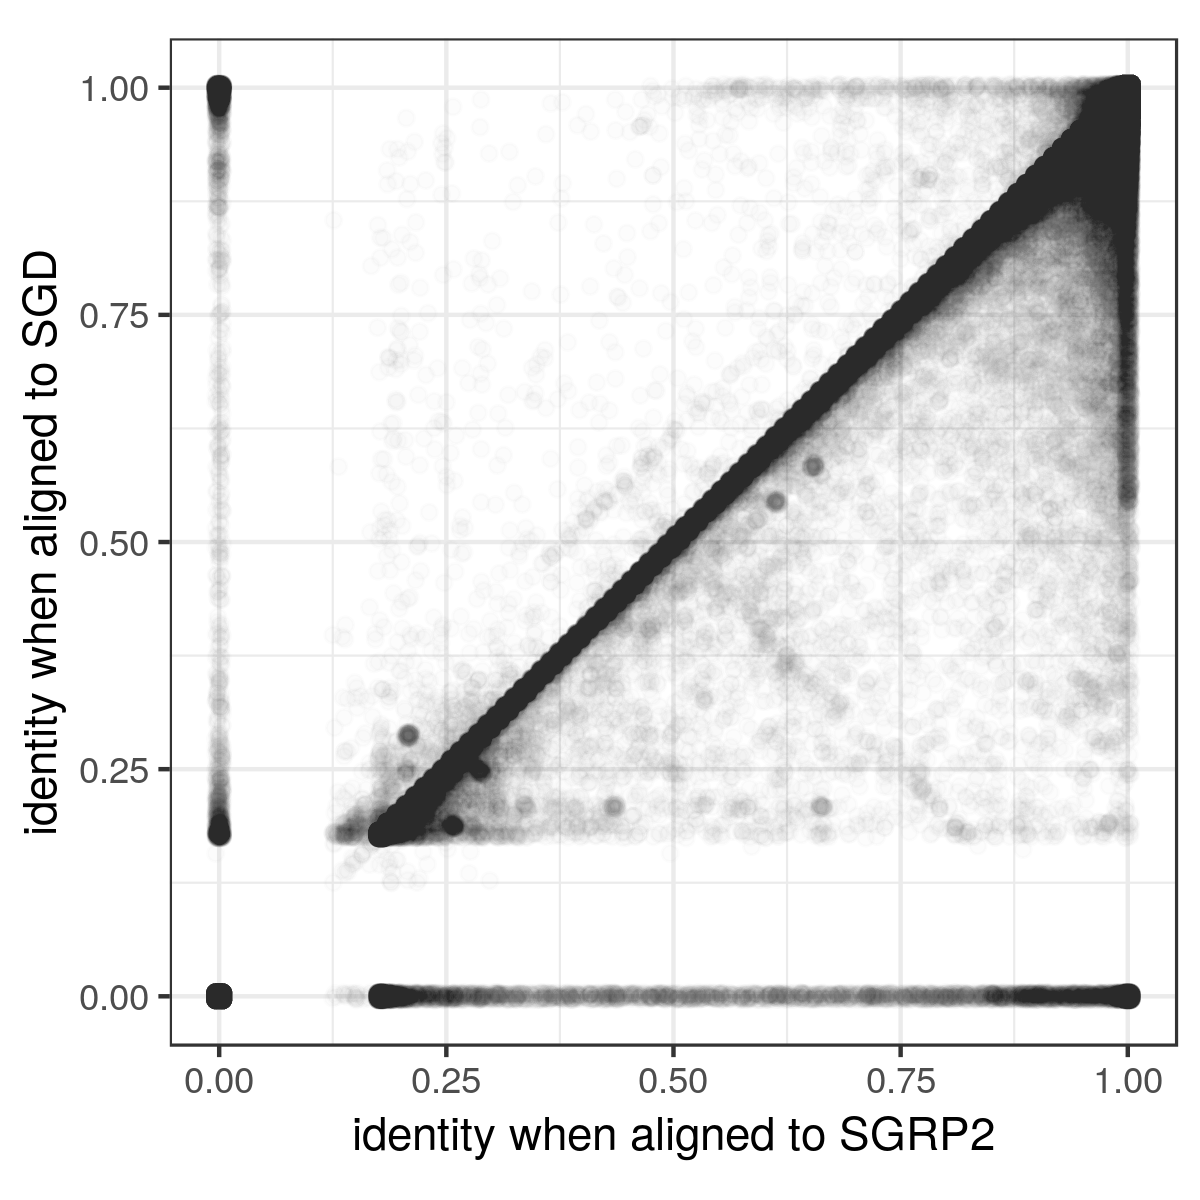
\includegraphics[width=1.0\textwidth]{Chapter3/Figs/NCYC_SGRP2_SGD_comparison_id.png}
    \caption{Alignment identity} \label{subfig:NCYC_identity}
  \end{subfigure}
  \begin{subfigure}[t]{1.0\textwidth}
    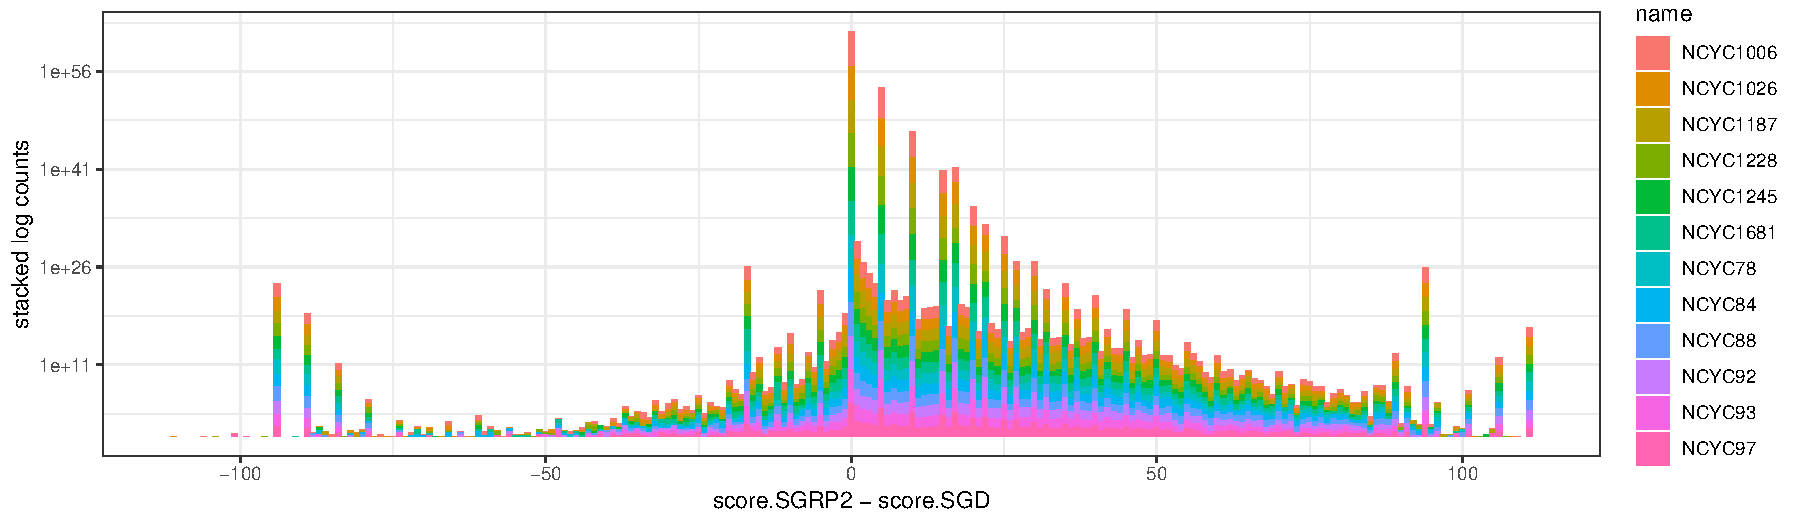
\includegraphics[width=1.0\textwidth]{Chapter3/Figs/NCYC_SGRP2_SGD_comparison_score_hist_color.pdf}
    \caption{Difference in alignment score} \label{subfig:NCYC_score_diff_hist}
  \end{subfigure}
  \begin{subfigure}[t]{1.0\textwidth}
    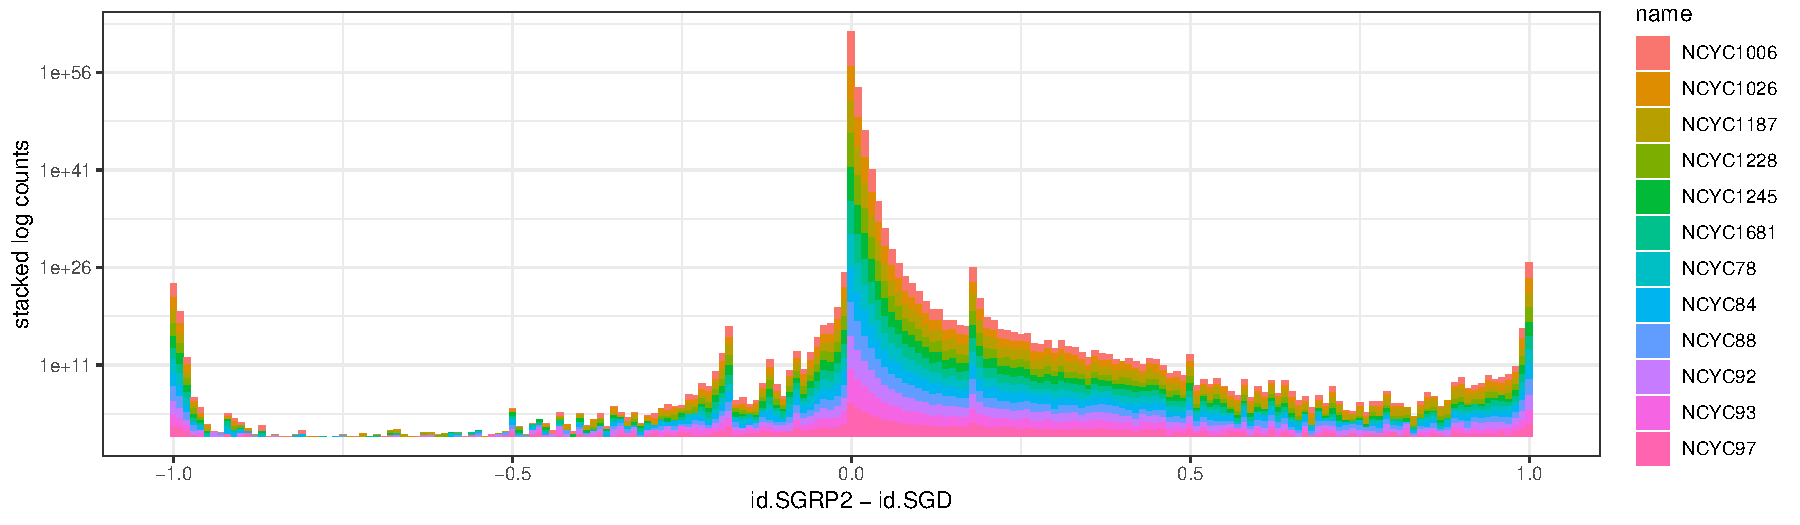
\includegraphics[width=1.0\textwidth]{Chapter3/Figs/NCYC_SGRP2_SGD_comparison_id_hist_color.pdf}
    \caption{Difference in alignment identity} \label{subfig:NCYC_id_diff_hist}
  \end{subfigure}
  \caption[Comparing alignment to the linear reference and SGRP2]{
    Alignment of 100k read pairs from 12 NCYC \emph{S. cerevisiae} strains(NCYC1006, NCYC1026, NCYC1187, NCYC1228, NCYC1245, NCYC1681, NCYC78, NCYC84, NCYC88, NCYC92, NCYC93, NCYC97) against the SGD\_2010 reference genome (SGD) or the SGRP2 pangenome (SGRP2).
    In (\ref{subfig:NCYC_score}) alignment scores are plotted for each read.
    The shift in density to the right relative to $y=x$ indicates improved alignments to the pangenome.
    In (\ref{subfig:NCYC_identity}) we observe the same pattern when using identity, or the fraction of the alignment which exactly matches the reference system.
    Subfigures \ref{subfig:NCYC_score_diff_hist} and \ref{subfig:NCYC_id_diff_hist} provide a log-scaled histogram of the difference in score and identity between the two graphs.
  }
\label{fig:NCYC_SGD_SGRP2}
\end{figure}

\subsection{Cactus progressive assembly}
%*0.5p 0.5h*


\begin{figure}[htbp!] 
  \centering
  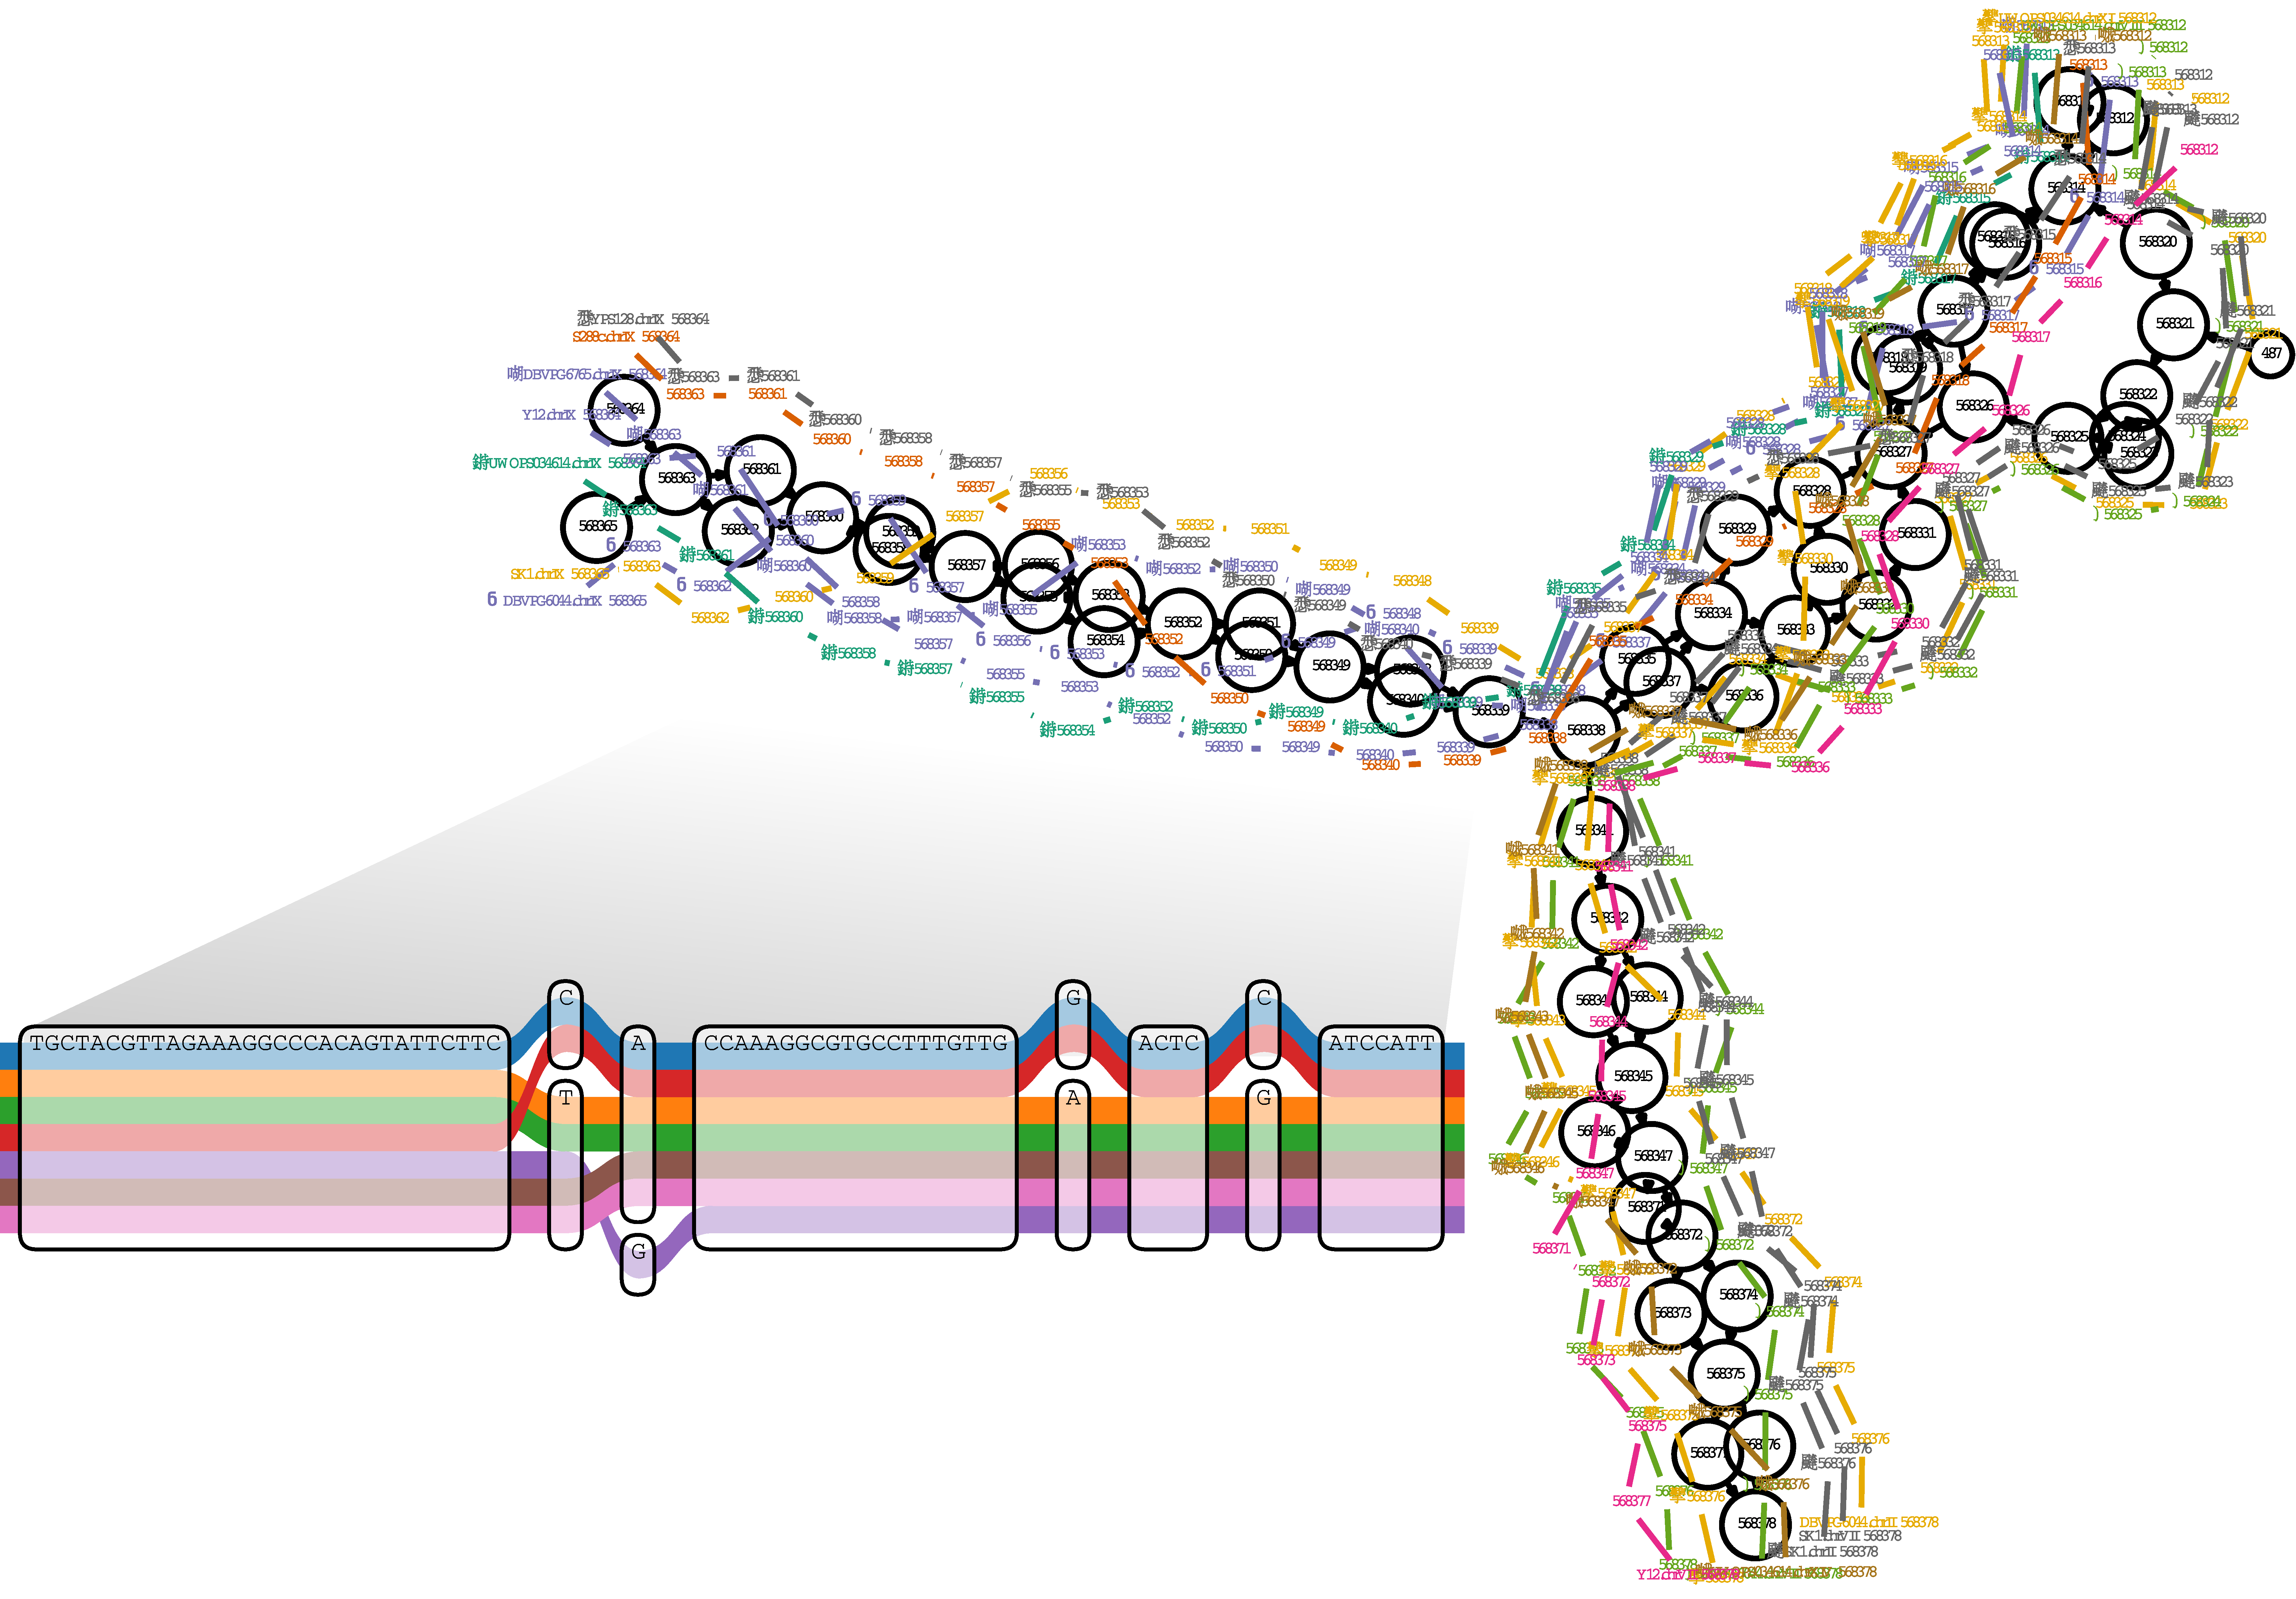
\includegraphics[width=1.0\textwidth]{Chapter3/Figs/cactus_yeast_zoom.pdf}
  \caption{
    A region of a yeast genome variation graph. This displays the start of the subtelomeric region on the left arm of chromosome 9 in a multiple alignment of the strains sequenced in \cite{yue2017contrasting} , built using vg from a full-genome multiple alignment generated with the Cactus alignment package \cite{Paten:2011fva}.
    The inset shows a subregion of the alignment at single-base level. The colored paths correspond to separate contiguous chromosomal segments of these strains.
    This illustrates the ability of vg to represent paths corresponding to both colinear (inset) and structurally rearranged (main figure) regions of genomic variation.
    }
  \label{fig:cactus_yeast_zoom}
\end{figure}

\begin{figure}[htbp!] 
  \centering
  \begin{subfigure}[t]{0.57\textwidth}
    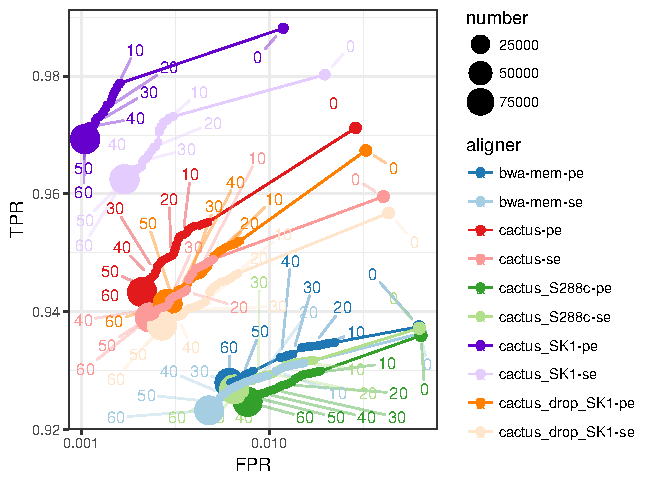
\includegraphics[width=1.0\textwidth]{Chapter3/Figs/e68fc338_test_sim_yeast_cactus-roc.pdf}
    \caption{Cactus yeast simulation} \label{subfig:cactus_sim}
  \end{subfigure}
  \begin{subfigure}[t]{0.42\textwidth}
    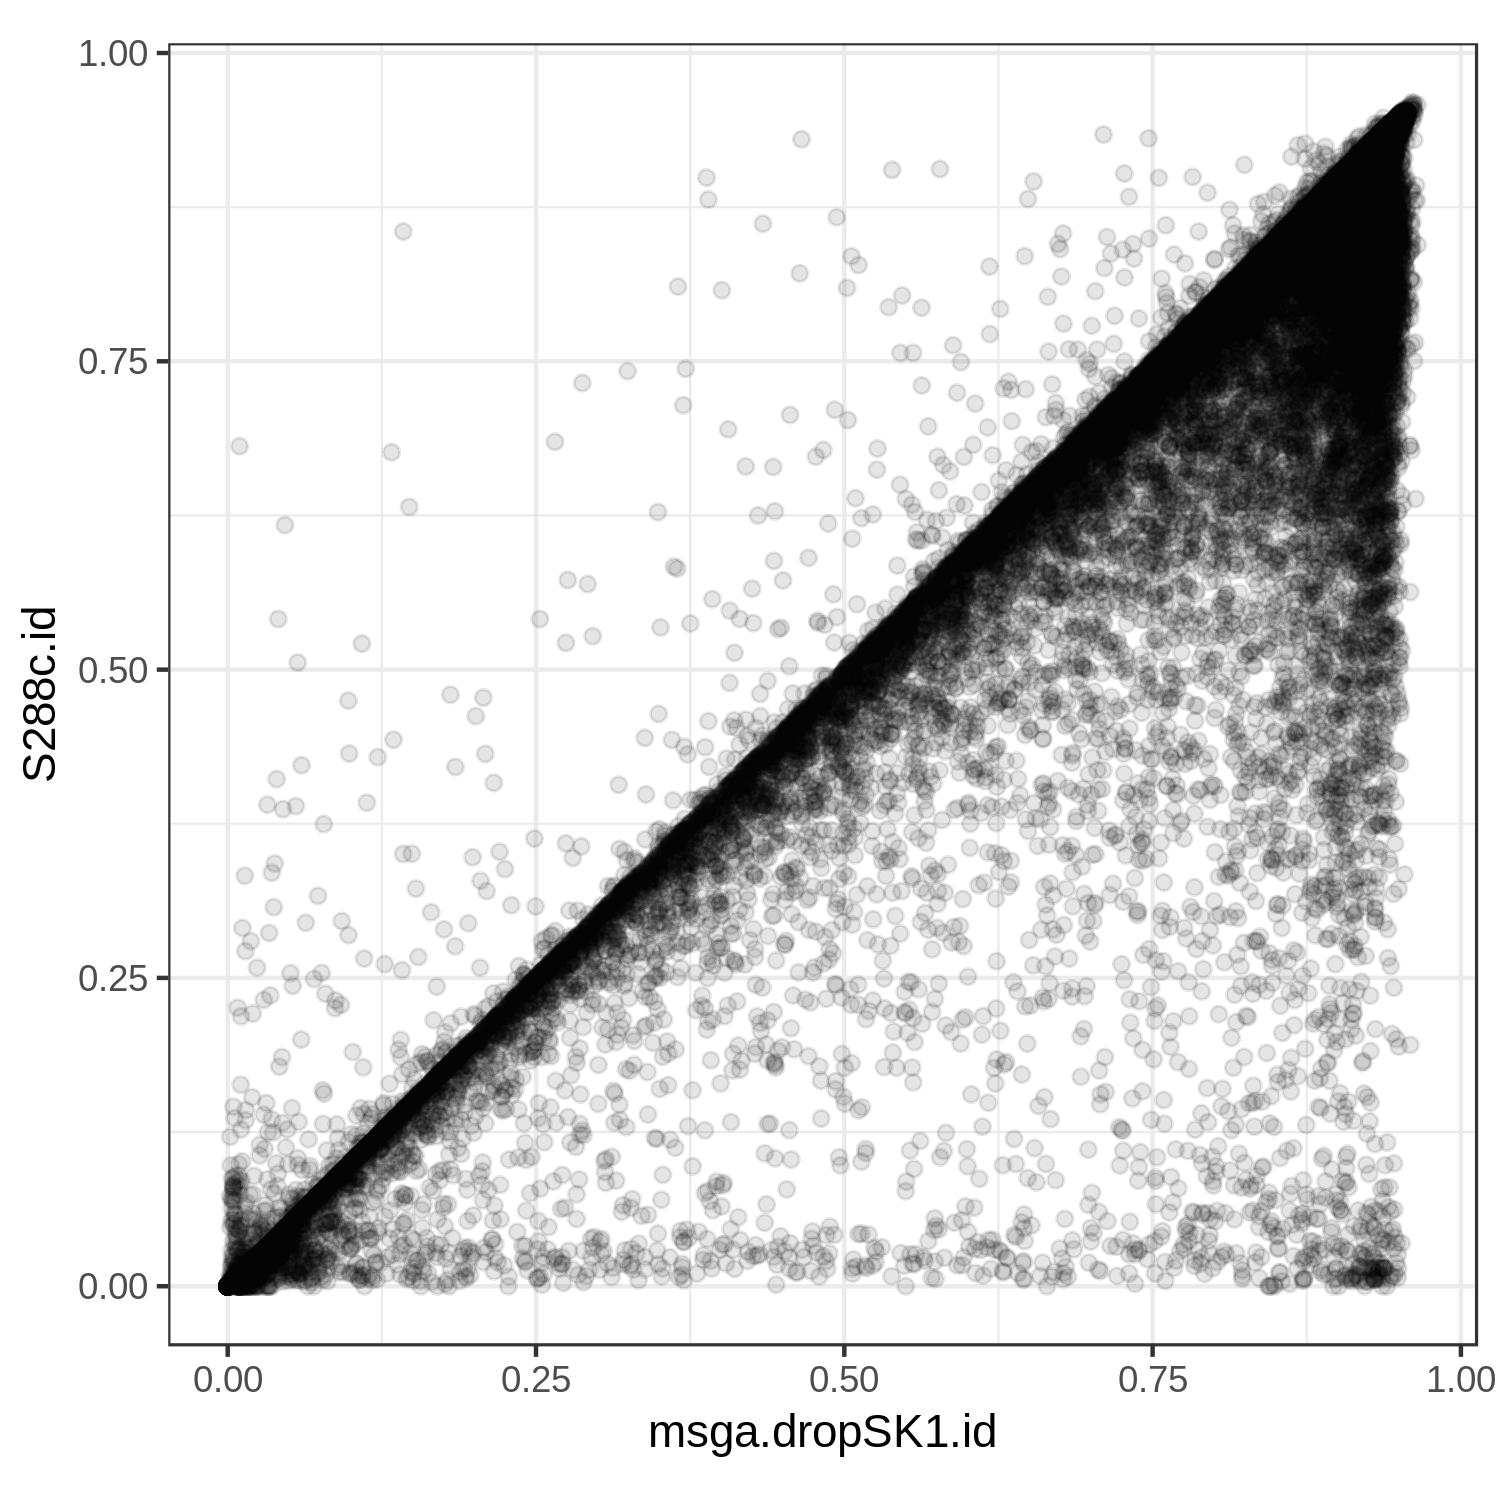
\includegraphics[width=1.0\textwidth]{Chapter3/Figs/compare-msga_dropSK1_vs_S288c.png}
    \caption{MSGA yeast holdout} \label{subfig:msga_SK1}
  \end{subfigure}
  \caption{Mapping short and long reads with vg to yeast genome references.
    (\ref{subfig:cactus_sim}) ROC curves obtained by mapping 100,000 simulated SK1 yeast strain 150-bp paired-end reads against a variety of references described in the text.
    (\ref{subfig:msga_SK1}) A density plot of identity fraction when mapping 43,337 Pacific Biosciences long reads from the SK1 strain to the drop.SK1 reference graph or the S288c reference.}
  \label{fig:yeast_generic_graphs}
\end{figure}

\subsection{Constructing and comparing variation graphs from whole genome assemblies}
%*3p 2.5h*

\subsection{Long read mapping} % from paper / my experiments

\section{Human}
%*0.5p 0.5h*

For a species such as human, with only 0.1\% nucleotide divergence on average between individual genome sequences, over 90\% of 100-bp reads will derive from sequence exactly matching the reference.
Therefore, new mappers should perform at least as well for linear reference mapping as the current standard, which we take to be {\tt bwa mem} with default parameters.
We show that vg does this, and then that vg maps more informatively around divergent sites.

\subsection{1000GP graph construction and indexing}
%*3p 3h*

The final phase of the 1000 Genomes Project (1000GP) produced a data set of ~80 million variants in 2,504 humans 16.
We made a series of vg graphs containing all variants or those with minor allele frequency thresholds at 0.1\%, 1\%, or 10\%, as well as a graph corresponding to the standard GRCh37 linear reference sequence without any variation.
The full vg graph uses 3.92 GB when serialized to disk, and contains 3.181 Gbp of sequence, which is exactly equivalent to the length of the input reference plus the length of the novel alleles in the VCF file.
Complete file sizes including indices range from 25 GB to 63 GB, with details including build and mapping times given in table \ref{table:1000GP}.

\begin{table}[h]
\begin{tabular}{l||c|cc|cc|cc}
\itshape Reference set & \itshape N vars & \multicolumn{2}{c}{\itshape vg} & \multicolumn{2}{c}{\itshape index} & \multicolumn{2}{c}{\itshape search time}\\
& \itshape (M) & \itshape time & \itshape size & \itshape time & \itshape size & \itshape  PE & \itshape SE\\
\hline
GRCh37 & 0 & 1:09:54 & 1.76 & 23:30:41 & 25.11 & 33:34 & 28:33 \\
1000GP AF0 & 84.8 & 3:42:01 & 3.92 & 51:05:07 & 63.28 & 45:10 & 39:46 \\
1000GP AF0.001 & 30.2 & 2:00:08 & 2.58 & 31:45:12 & 38.10 & 39:33 & 32:53 \\
1000GP AF0.01 & 14.3 & 1:35:02 & 2.17 & 27:18:53 & 30.94 & 33:13 & 27:09\\
1000GP AF0.1 & 6.8 & 1:23:04 & 1.97 & 26:06:38 & 27.79 & 32:35 & 28:43 \\
\hline
\end{tabular}
\caption{Numbers of variants, file sizes in gigabytes (GB) and build and search times in hours:minutes:seconds for various human vg graphs and associated indexes. Reference sets are the linear reference GRCh37, the full 1000 Genomes Project set 1000GP AF0, and subsets of 1000GP AF0 including only variants with allele frequency above thresholds 0.001 (0.1\%), 0.01 (1\%) and 0.1 (10\%) respectively.  The number of variants in millions for each of these data sets is shown.  Search times are for 10 million 150+150bp read pairs simulated from NA24385.
}
\label{table:1000GP}
\end{table}

\subsection{Simulations based on phased HG002}
\label{sec:1000GP_sim}

We next aligned ten million 150-bp paired-end reads simulated with errors from the parentally phased haplotypes of an Ashkenazi Jewish male NA24385, sequenced by the Genome in a Bottle (GIAB) Consortium \cite{zook2016extensive} and not included in the 1000GP sample set, to each of these graphs as well as to the linear reference using {\tt bwa mem}.
Figure \ref{fig:HG002_1000GP_sim} shows the accuracy of these alignments compared with {\tt bwa mem} for the the full range of frequency thresholded graph, in terms of receiver operating characteristic (ROC) curves.

Reads that come from parts of the sequence without differences from the reference (middle panels of Figure \ref{fig:HG002_1000GP_sim}) mapped slightly better to the reference sequence (green) than to the 1000GP graph (red), which we attribute to a combination of the increase in options for alternative places to map reads provided by the variation graph, and the fact that we needed to prune some search index $k$-mers in the most complex regions of the graph.
The best balance of performance appears at the threshold of 0.01, as in panel C.
As expected, this difference increased as the allele frequency threshold was lowered and more variants were included in the graph, as seen in Figure \ref{fig:HG002_1000GP_sim} panels A and B.

For reads that were simulated from segments containing non-reference alleles (~10\% of reads), which are the reads relevant to variant calling, {\tt vg} mapping to the 1000GP graph (red) gave better performance than either {\tt vg} (green) or {\tt bwa mem} (blue) mapping to the linear reference (right panels of Figure \ref{fig:HG002_1000GP_sim}), because many variants present in NA24385 are already represented in the 1000GP graph.
This is particularly clear for single-end mapping, since many paired-end reads are rescued by the mate read mapping.
Overall, vg performed at least as well as bwa mem, even on reference-derived reads, and substantially better on reads containing non-reference variants.

\begin{figure}[htbp!] 
\centering    
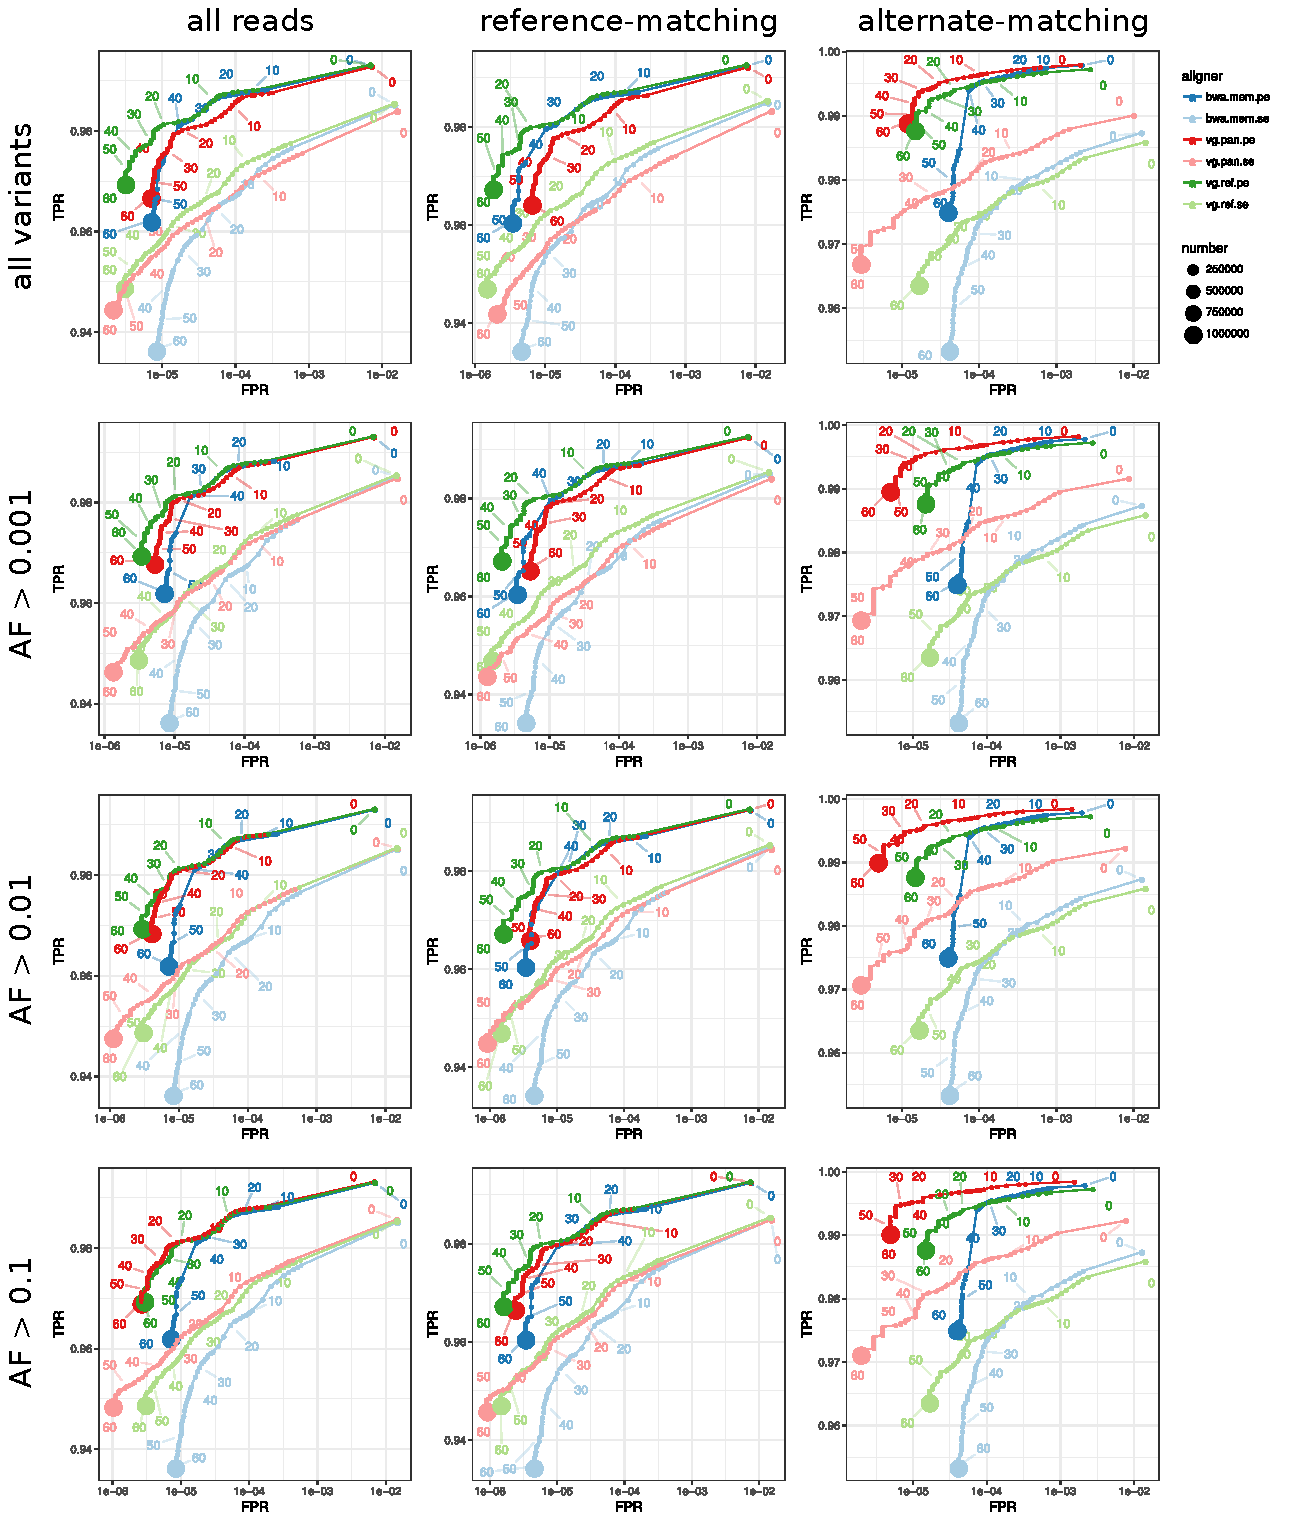
\includegraphics[width=1.0\textwidth]{Chapter3/Figs/human-10M-results-7358a67_merge_panel_labeled.pdf}
\caption[Simulated reads from HG002 versus various human pangenome graphs.]{
  ROC curves parameterised by mapping quality for 10M read pairs simulated from NA24385 as mapped by bwa mem, vg to various 1000GP pangenome references, and vg with a linear reference, using single end (se) or paired end (pe) mapping.
  Allele frequency thresholds for the various panels are A) all variants, B) 0.001, C) 0.01, and D) 0.1.
  Within each panel, the left subpanel is based on all reads, middle on reads simulated from segments with no genetic variants from the linear reference, right on reads simulated from segments containing variants.
  All reads may contain simulated sequencing errors reflecting SNPs at a rate of 0.01 per base and indels at a rate of 0.002 per base.}
\label{fig:HG002_1000GP_sim}
\end{figure}

\subsection{Aligning and analyzing a real genome}

We also mapped a real human genome read set with ~50× coverage of Illumina 150-bp paired-end reads from the NA24385 sample to the 1000GP graph. vg produced mappings for 98.7\% of the reads, 88.7\%
with reported mapping quality score 30 on the Phred scale, and 76.8\% with perfect, full-length sequence identity to the reported path on the graph.
For comparison, we also used vg to map these reads to the linear reference.
Similar proportions of reads mapped (98.7\%) and with reported quality score 30 (88.8\%), but considerably fewer with perfect identity (67.6\%).
Markedly different mappings were found for 1.0\% of reads (0.9\% mapping to widely separated positions on the two graphs, and 0.1\% mapping to one graph but not the other).
The reads mapping to widely separated positions were strongly enriched for repetitive DNA. For example, the linear reference mappings for 27.5\% of these read pairs overlapped various types of satellite DNA identified by RepeatMasker, compared to 3.0\% of all read pairs.

To illustrate the consequences of mapping to a reference graph rather than a linear reference, we stratified the sites independently called as heterozygous in NA24385 by deletion or insertion length (0 for single-nucleotide variants) and by whether the site was present in 1000GP, and measured the fraction of reads mapped to the alternate allele for each category.
The results show that mapping with vg to the population graph when the variant was present in 1000GP (95.4\% of sites) gave nearly balanced coverage of alternate and reference alleles independent of variant size, whereas mapping to the linear reference either with {\tt vg} or {\tt bwa mem} led to a progressively increasing bias with increasing deletion and (especially) insertion length (Figure \ref{fig:HG002_indels}), so that for insertions around 30 bp, a majority of insertions containing reads were missing (there were over twice as many reference reads as alternate reads).

\begin{figure}[htbp!] 
\centering    
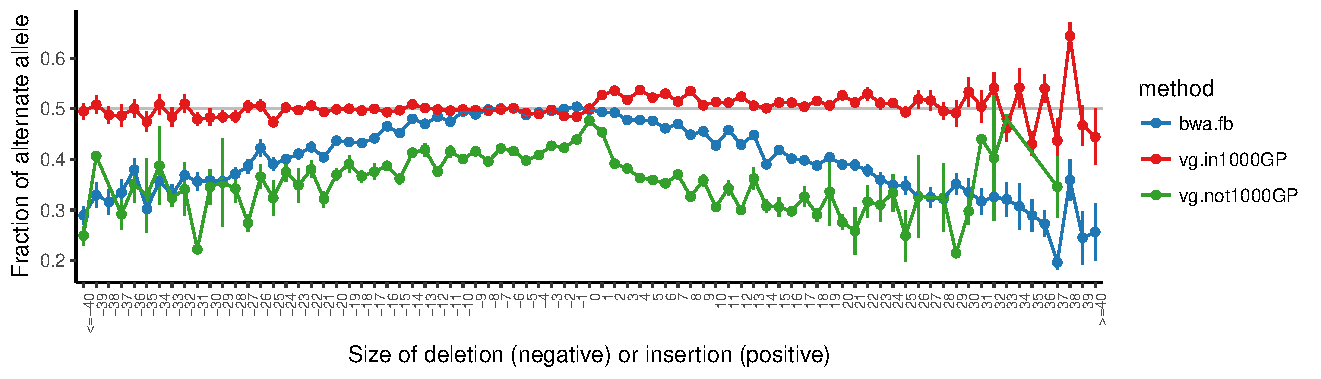
\includegraphics[width=1.0\textwidth]{Chapter3/Figs/HG002_wg_pan_ref_bwa_true_hets_allele_balance_tsv_gz_3.pdf}
\caption[Indel allele balance in HG002]{The mean alternate allele fraction at heterozygous variants previously called in HG002/NA24385 as a function of deletion or insertion size (SNPs at 0). Error bars are ± 1 s.e.m.}
\label{fig:HG002_indels}
\end{figure}

\subsection{Whole genome variant calling experiments}

We explored the application of {\tt vg} to whole genome alignment and variant calling in the PrecisionFDATruth Challenge, in which the team which developed the Genome in a Bottle truth set developed and held out a new sample.
Methods were first tested against publicly available truth sets on NA12878 in the ``consistency'' challenge, in which the {\tt vg} development team received a star for ``heroic effort'' in completing the first whole-genome graph based alignment and variant calling analysis.
The results for this first iteration were very poor, with F-scores for indels and SNPs around 95\%.
The computational costs were high, with the run consuming around \$1000 in resources on Amazon's Elastic Compute cloud (AWS EC2).

In the final round of the challenge, we obtained results as described in table \ref{table:PFDA}.
We find that the {\tt vg} pipeline had similar performance to the \emph{de novo} assembly pipeline fermikit for SNPs.
Methods that are not explicitly based on the GATK indel calling method perform notably worse on indels, including egarrison-hhga\footnote{This was my work along with Nicolas Della Penna, \url{https://github.com/ekg/hhga}. Unfortunately, it remains unpublished.}, which used Platypus, fermikit, and freebayes to generate candidate variants and implemented a genotyper using a machine learning method, and mlin-fermikit, which was a direct application of fermikit's standard pipeline to the data for HG002.
However, {\tt vg call}'s indel calling results were very poor, and likely caused by bugs in the variant caller and aligner at this stage rather than conceptual problems with graph based variant calling.

\begin{table}[h]
\begin{tabular}{l||ccc|ccc}
\itshape Submission & \multicolumn{3}{c}{\itshape SNPs} & \multicolumn{3}{c}{\itshape indels}\\
& \itshape F-score & \itshape recall & \itshape precision & \itshape F-score & \itshape recall & \itshape precision \\
\hline
anovak-vg & 98.4545 & 98.3357 & 98.5736 & 70.4960 & 69.7491 & 71.2591 \\
astatham-gatk & 99.5934 & 99.2091 & 99.9807 & 99.3424 & 99.2404 & 99.4446 \\
bgallagher-sentieon & 99.9296 & 99.9673 & 99.8919 & 99.2678 & 99.2143 & 99.3213 \\
dgrover-gatk & 99.9456 & 99.9631 & 99.9282 & 99.4009 & 99.3458 & 99.4561 \\
egarrison-hhga & 99.8985 & 99.8365 & 99.9607 & 97.4253 & 97.1646 & 97.6874 \\
hfeng-pmm3 & 99.9548 & 99.9339 & 99.9756 & 99.3628 & 99.0161 & 99.7120 \\
mlin-fermikit & 98.8629 & 98.2311 & 99.5029 & 95.5997 & 94.8918 & 96.3183 \\
rpoplin-dv42 & 99.9587 & 99.9447 & 99.9728 & 98.9802 & 98.7882 & 99.1728 \\
\hline
\end{tabular}
\caption{A selected subset of PrecisionFDA Truth Challenge results showing the best-performing methods as well as a number of other notable submissions.}
\label{table:PFDA}
\end{table}

We also explored integration of vg with the recently published GraphTyper \cite{eggertsson2017graphtyper} method, which calls genotypes by remapping reads to a local, partially ordered variation graph built from a VCF file, relying on initial global assignment to a region of the genome by mapping with bwa to a linear reference.
Therefore, although GraphTyper also scales to the whole human genome because it is essentially a local method, its functionality is complementary to that of vg, which maps to a global variation graph and does not directly call genotypes.
In experiments where we used vg rather than bwa as the primary mapper for GraphTyper, true positives increased marginally (0.02\% for single-nucleotide polymorphisms (SNPs) and 0.06\% for indels) while false positives increased for SNPs by 0.15\% and decreased for indels by 0.03\%.
We note, however, that GraphTyper was developed by its authors for {\tt bwa mem} mapping.

\subsection{HGSVC from VCF and progressive alignment of human chromosomes}
%*2.5p 5h*


\subsection{CHiP-Seq}
%*1p 1h*

This removal of bias is important when mapping functional genomics data such as ChIP-seq data, where allele-specific expression analysis can reveal genetic variation that affects function but is confounded
by reference mapping bias \cite{mcdaniell2010heritable}, especially given that read lengths are typically shorter for these experiments.
We compared mapping with {\tt bwa mem} and {\tt vg} for data set ENCFF000ATK from the ENCODE project \cite{encode2012integrated}, which contains 14.9 million 51-bp ChIP-seq reads for the H3K4me1 histone methylation mark from the NA12878 cell line.
When mapping with bwa the ratio of reference to alternate allele matches at heterozygous sites was 1.20, whereas with vg to the 1000GP graph the ratio was 1.01, effectively eliminating reference bias.

\section{Ancient DNA}
%*0.5p 0.5h*
With aDNA, read lengths are limited by the degredation of DNA due to environmental exposure.
Furthermore, degredation causes a high intrinsic error rate.
In combination these issues cause a strong bias against non-reference variation.
This has significant effect on population genetic inference and implications for many aDNA studies.

\subsection{Simulations with human origins panel}
%*1p 2h*

\subsection{Using 1000GP graph for samples from Martiniano et al 2016}
%*2p 4h*

\subsection{Evaluation of a high-coverage Botai sample}
%*2p 4h*


\section{Neoclassical bacterial pangenomics}
%*0.5p 0.5h*

\subsection{E. coli pangenome from illumina reads}
%*2p 4h*

\subsection{Evaluating the core and accessory pangenome}
%*2p 4h*


\section{Metagenomics}
%*0.5p 0.5h*

\subsection{Arctic viral metagenome}
%*2p 1.5h*

\subsection{Human gut microbiome}
%*2p 8h*


\section{RNAseq}
%*0.5p 0.5h*

\subsection{Yeast}
%*1p 2h*

\subsection{C. elegans}
%*2p 5h*

\subsection{Human}
%*2p 12h*


\section{Applications that I contributed to}

% ...
